\begin{adjustbox}{max width=\textwidth, max totalheight=0.6\textheight, center}
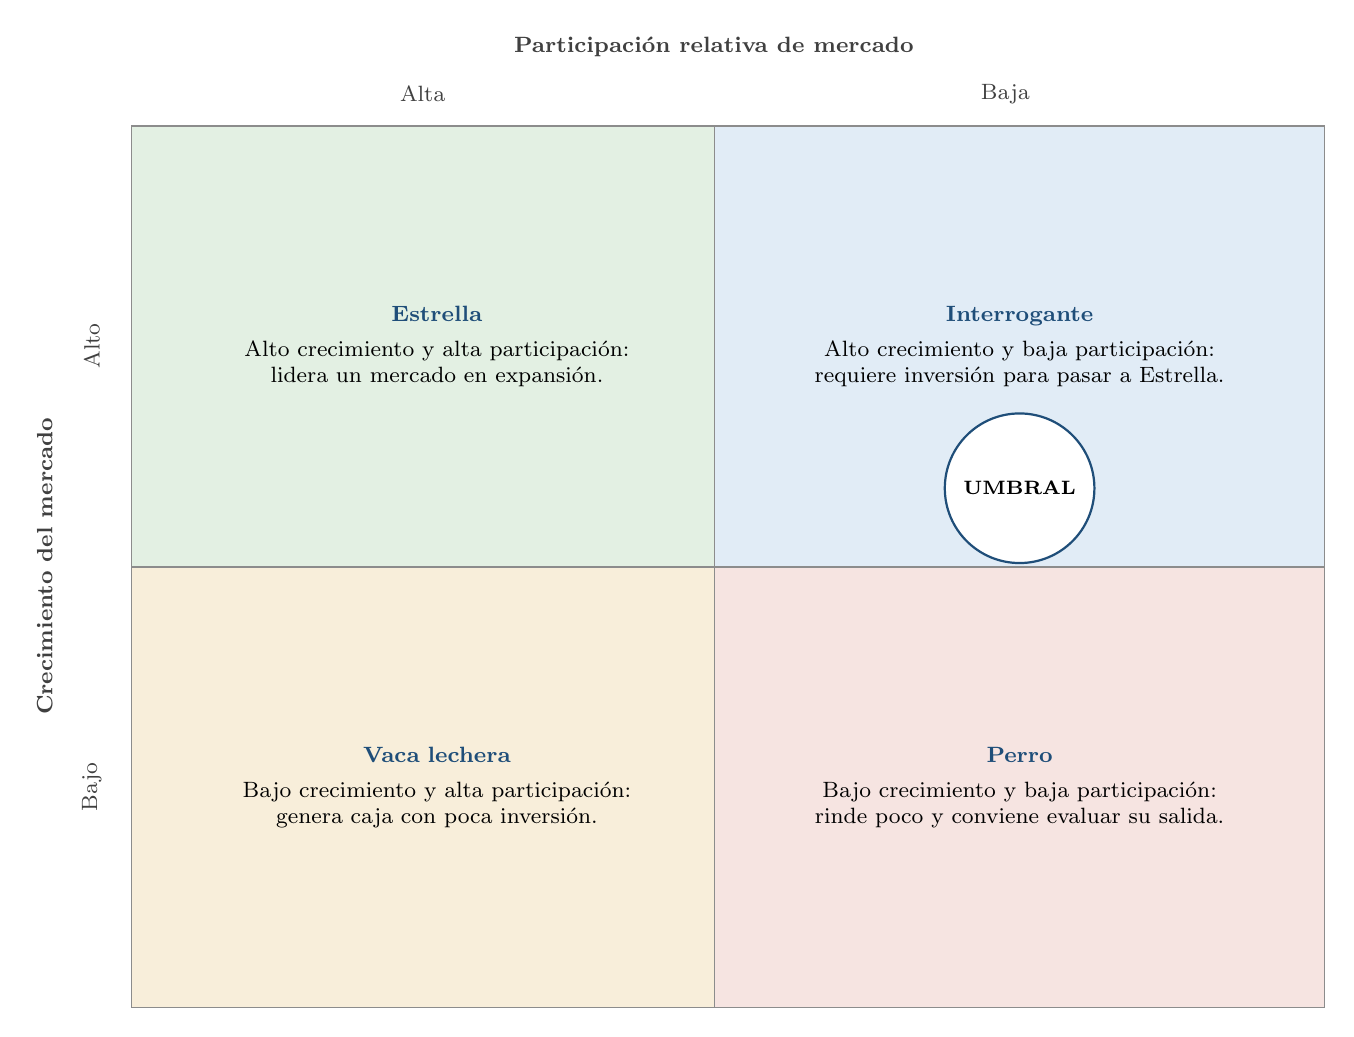
\begin{tikzpicture}[x=1cm, y=1cm]
% Estilos comunes de las figuras TikZ (despliegue y modelo relacional).
\definecolor{acento}{HTML}{1F4E79}
\hyphenpenalty=10000 \exhyphenpenalty=10000
\tikzset{
	caja/.style={draw=black!60, line width=0.4pt, fill=white, rounded corners=1pt, align=center, font=\footnotesize, inner sep=4pt, minimum height=0.9cm, text width=3.2cm},
	cajaacento/.style={caja, draw=acento, line width=0.7pt},
	opc/.style={caja, dashed, draw=black!55},
	almacen/.style={draw=black!60, line width=0.4pt, fill=black!6, cylinder, shape border rotate=90, aspect=0.22, align=center, font=\footnotesize, inner sep=3pt, minimum height=1.5cm, text width=2.6cm},
	zona/.style={draw=black!45, line width=0.4pt, fill=black!3, rounded corners=2pt, inner sep=8pt},
	zonaint/.style={draw=black!45, line width=0.4pt, fill=white, rounded corners=2pt, inner sep=7pt},
	flecha/.style={-{Stealth[length=5pt,width=4pt]}, line width=0.5pt, draw=black!70},
	rotulo/.style={font=\scriptsize, fill=white, inner sep=1.5pt},
	titulo/.style={font=\footnotesize\bfseries, text=black!75, anchor=south west},
}

\definecolor{cF}{HTML}{E3F0E3}\definecolor{cD}{HTML}{F6E4E1}\definecolor{cO}{HTML}{E1ECF6}\definecolor{cA}{HTML}{F8EEDA}
\tikzset{cuad/.style={draw=black!45, line width=0.4pt, inner sep=5pt, anchor=north west, font=\footnotesize, text width=7.4cm, align=center, minimum height=5.6cm},
 eje/.style={font=\footnotesize\bfseries, text=black!75, align=center},
 niv/.style={font=\footnotesize, text=black!75}}
\node[cuad, fill=cF] (E) at (0,0) {\textbf{\textcolor{acento}{Estrella}}\\[3pt]Alto crecimiento y alta participación: lidera un mercado en expansión.};
\node[cuad, fill=cO] (I) at (7.4,0) {\textbf{\textcolor{acento}{Interrogante}}\\[3pt]Alto crecimiento y baja participación: requiere inversión para pasar a Estrella.};
\node[cuad, fill=cA] (V) at (0,-5.6) {\textbf{\textcolor{acento}{Vaca lechera}}\\[3pt]Bajo crecimiento y alta participación: genera caja con poca inversión.};
\node[cuad, fill=cD] (P) at (7.4,-5.6) {\textbf{\textcolor{acento}{Perro}}\\[3pt]Bajo crecimiento y baja participación: rinde poco y conviene evaluar su salida.};
\node[draw=acento, line width=0.8pt, fill=white, circle, inner sep=2pt, minimum size=1.9cm, font=\scriptsize\bfseries] at ([yshift=-1.8cm]I.center) {UMBRAL};
\node[niv, rotate=90] at (-0.5,-2.8) {Alto};
\node[niv, rotate=90] at (-0.5,-8.4) {Bajo};
\node[eje, rotate=90] at (-1.1,-5.6) {Crecimiento del mercado};
\node[niv] at (3.7,0.4) {Alta};
\node[niv] at (11.1,0.4) {Baja};
\node[eje] at (7.4,1.0) {Participación relativa de mercado};
\end{tikzpicture}
\end{adjustbox}
